\chapter{Implementación\label{cap:implementacion}}

TODO: [Introducción]


\section{Back-End\label{sec:imp:back_end}}

Introducción implementación back-end

Stack de librerías: io.js, express, supervisor, apiDoc

1 párrafo: servicio instalado que se autoinicia

\begin{figure}[!htp]
  \centering
  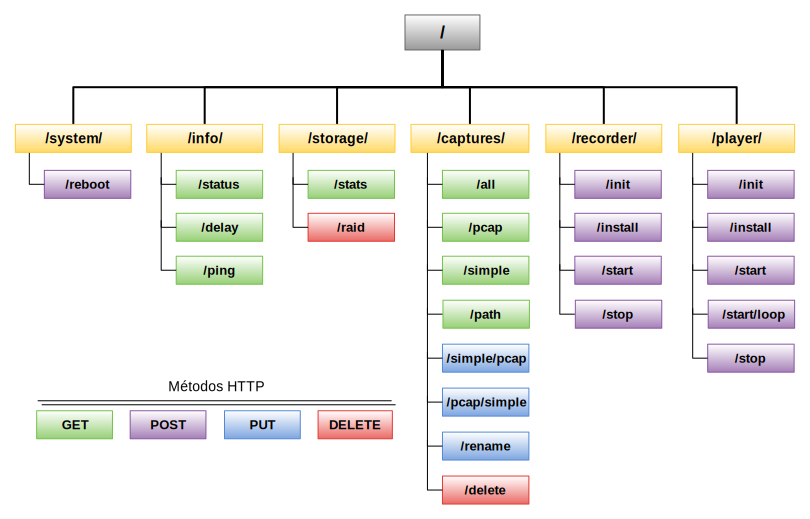
\includegraphics[width=\textwidth,clip=true]{arbol_metodos}
  \caption{Métodos públicos del \gls{servicioweb} \gls{FPGA}.}
  \label{fig:arbol_metodos}
\end{figure}

Arbol rutas~\ref{fig:fpga_estado}

\begin{figure}[!htp]
  \centering
  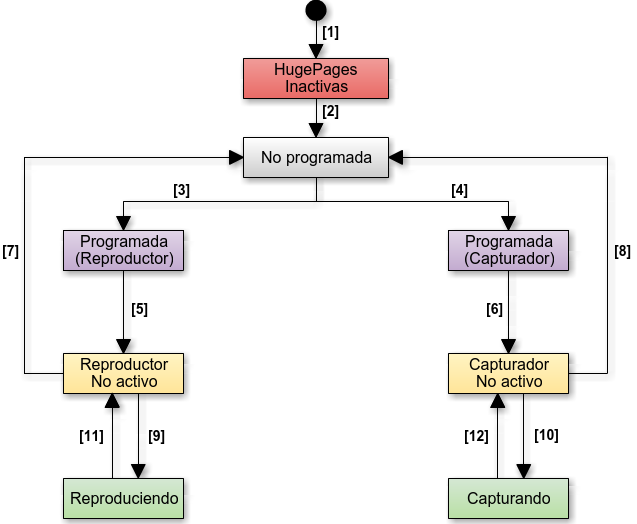
\includegraphics[width=\textwidth,clip=true]{fpga_estado}
  \caption{Máquina de Estados Finita para el estado de la \gls{FPGA}.}
  \label{fig:fpga_estado}
\end{figure}

FSM de estados FPGA~\ref{fig:fpga_estado}

cuando llega una petición que depende del estado, primero se determina el estado. Para esto se van realizando tests de forma incremental etc. árbol de transiciones,~\ref{fig:arbol_decision}

\begin{figure}[!htp]
  \centering
  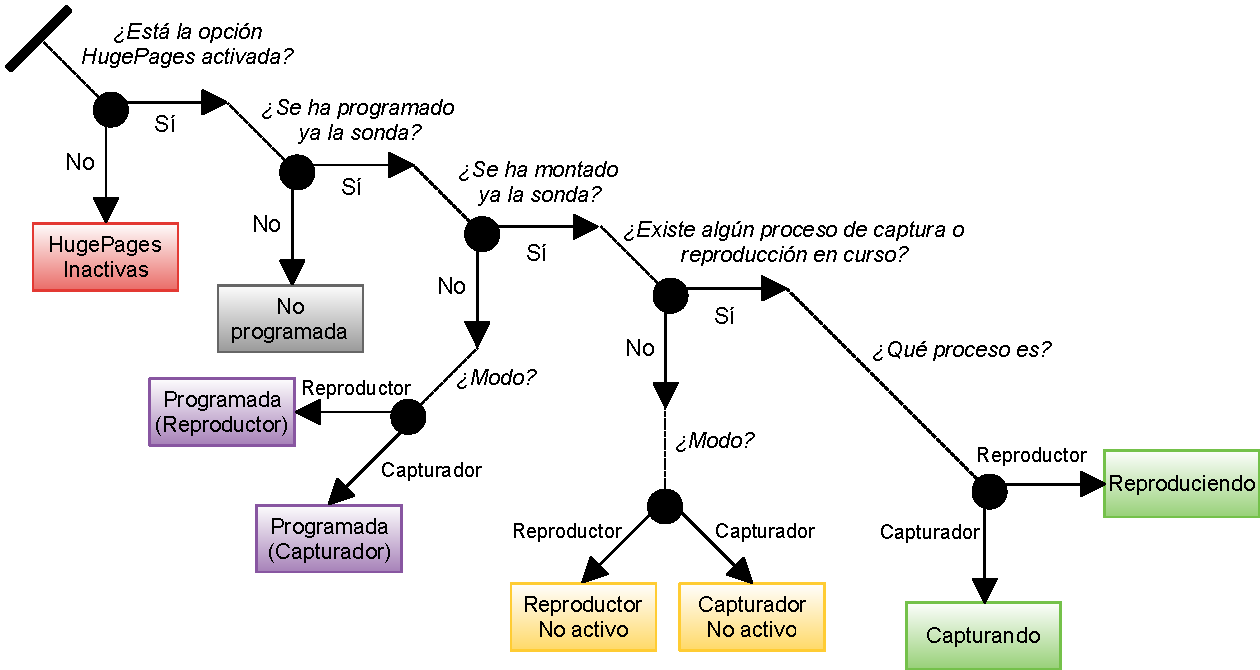
\includegraphics[width=0.75\textwidth,clip=true]{arbol_decision}
  \caption{Árbol de decisión para determinar el estado de la \gls{FPGA}.}
  \label{fig:arbol_decision}
\end{figure}
es necesario puesto que el servidor es stateless

Internamente, las transiciones
\begin{enumerate}[label={\bfseries [\arabic*]}]
  \item Estado por defecto al iniciar el servidor sin seleccionar la opción de arranque con \textit{HugePages}.
  \item Se reinicia el servidor, seleccionando la opción de arranque con la opción \textit{HugePages} activa.
  \item Se programa la \gls{FPGA} en modo reproductor con el \gls{bitstream} correspondiente y se reinicia el servidor.
  \item Se programa la \gls{FPGA} en modo capturador con el \gls{bitstream} correspondiente y se reinicia el servidor.
  \item Se monta la \gls{FPGA} sobre el servidor.
  \item Se monta la \gls{FPGA} sobre el servidor.
  \item Se reinicia el servidor.
  \item Se reinicia el servidor.
  \item Se ordena a la sonda reproducir una \gls{traza}.
  \item Se ordena a la sonda capturar una \gls{traza}.
  \item Se para la reproducción, o porque se ha acabado el contenido de la \gls{traza} o porque es detenida el usuario.
  \item Se para la captura, o porque se ha capturado todo lo que se quería o porque es detenida por el usuario.
\end{enumerate}


Captura árbol de archivos~\ref{fig:arbol_codigo}

\begin{figure}[!htp]
  \begin{center}
    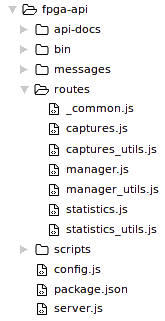
\includegraphics[width=0.3\textwidth,clip=true]{capturas/arbol_backend}
    \hspace{1cm}
    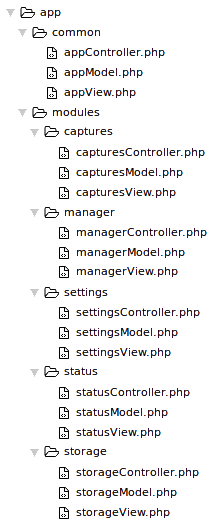
\includegraphics[width=0.3\textwidth,clip=true]{capturas/arbol_frontend}
  \caption{Árboles con los principales archivos de código del \gls{back-end} (a la izquierda) y del \gls{front-end} (a la derecha).}
  \label{fig:arbol_codigo}
  \end{center}
\end{figure}


\section{Front-End\label{sec:imp:front_end}}

Introducción

Resultado Capturas diseño responsive (misma página desde dos sitios)~\ref{fig:captura:movil}
\begin{figure}[!htp]
  \centering
  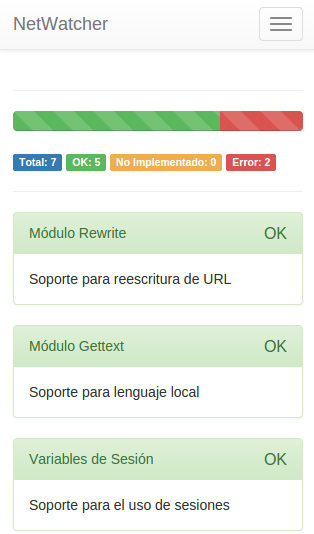
\includegraphics[width=0.4\textwidth,clip=true]{capturas/estado_movil}
  \caption{Página de la aplicación visualizada desde un dispositivo móvil.}
  \label{fig:captura:movil}
\end{figure}

Stack de librerías: MVC propio,Bootstrap,jQuery,gettext, etc.

Captura árbol de archivos~\ref{fig:arbol_codigo}

Internacionalización

Temas (captura algún temas)~\ref{fig:captura:oscuro}
\begin{figure}[!htp]
  \centering
  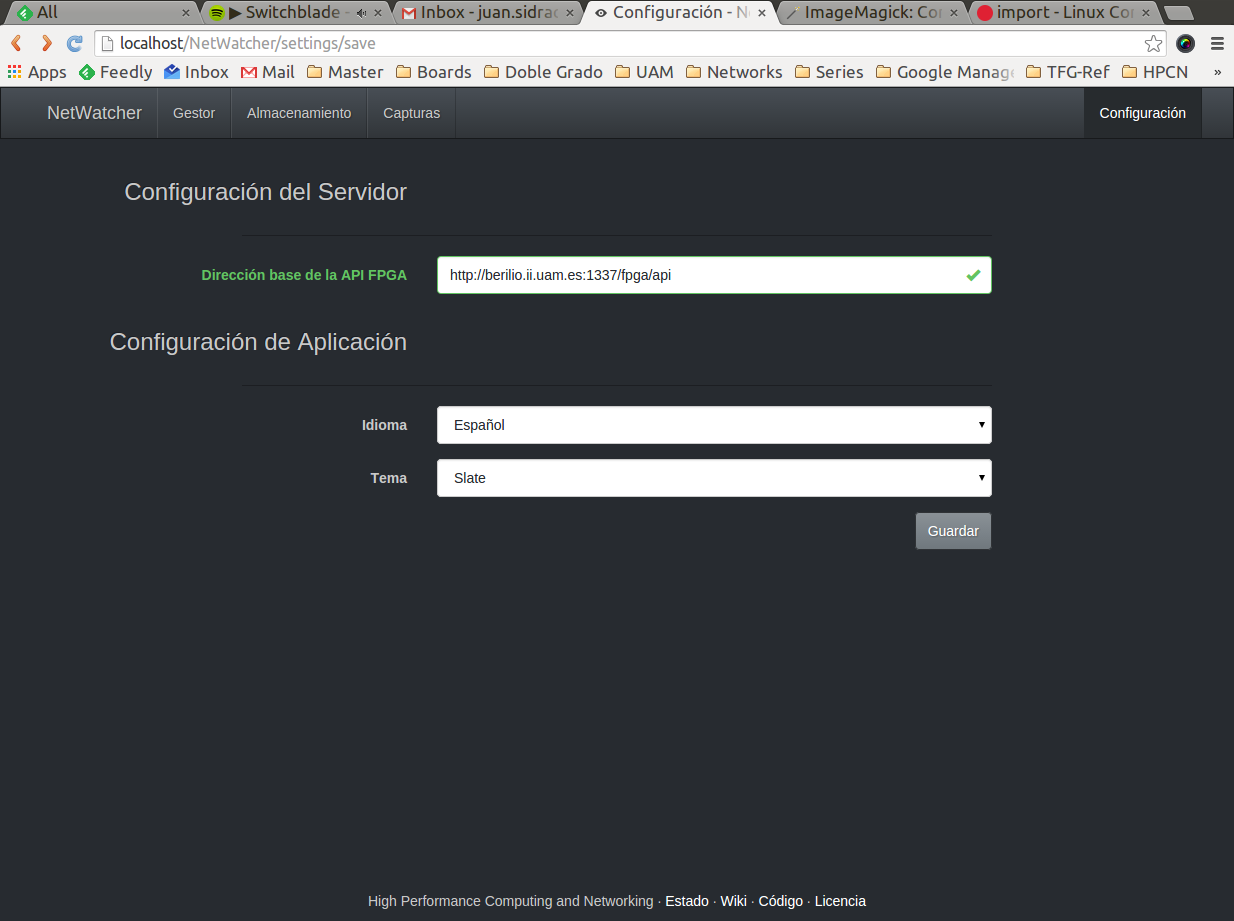
\includegraphics[width=0.95\textwidth,clip=true]{capturas/configuracion_tema_oscuro}
  \caption{Página de la aplicación con un tema oscuro seleccionado.}
  \label{fig:captura:oscuro}
\end{figure}


\section{Documentación \label{sec:imp:docs}}

Se ha creado distinta documentación del proyecto según a quién esté dirigida.
Por un lado, se ha escrito un manual de usuario (disponible en el apéndice~\ref{extra:manual_de_usuario}), que pretende ser una guía completa y suficiente para la instalación, configuración y uso de la aplicación.
Adicionalmente, se han publicado en el repositorio de \textit{GitHub} del proyecto (\url{github.com/JSidrach/NetWatcher}) una serie de páginas en formato \textit{wiki} (ver Figura~\ref{fig:captura:wiki}). Estas páginas, en inglés, recogen los aspectos más importantes de la aplicación, tanto para el usuario final como para desarrolladores.

\begin{figure}[!htp]
  \centering
  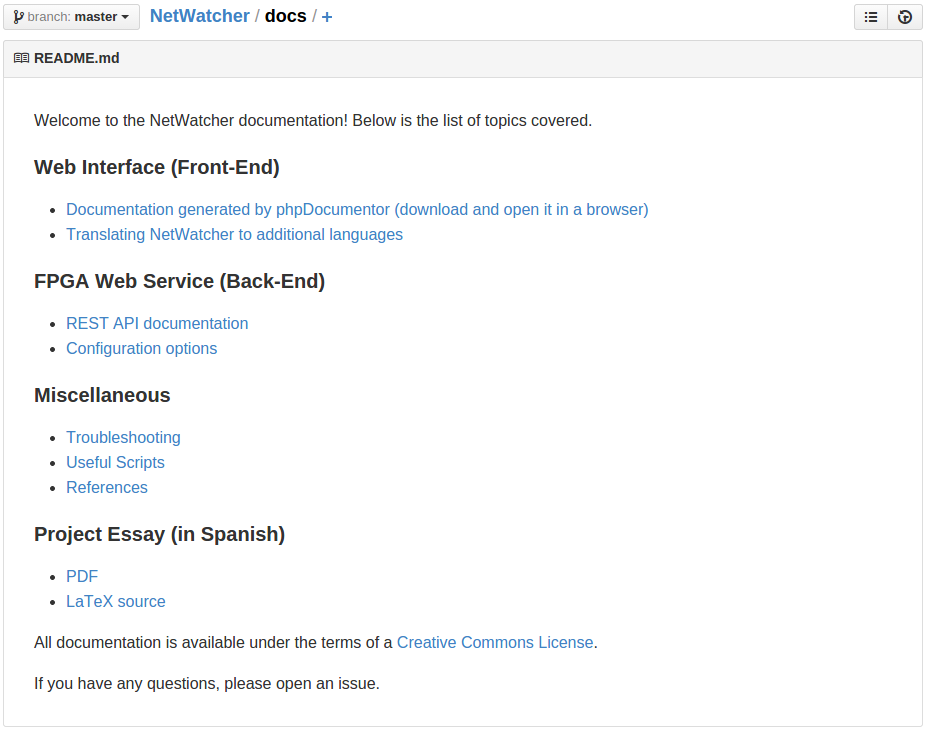
\includegraphics[width=0.95\textwidth,clip=true]{graphics/capturas/github_docs}
  \caption{Captura de una de las páginas de la wiki del proyecto.}
  \label{fig:captura:wiki}
\end{figure} 

A nivel específico de desarrollador, se han utilizado dos herramientas para crear la documentación interna, accesible a través del navegador y en inglés. 
La documentación del \gls{front-end} se ha generado con \textit{phpDocumentor} (ver Figura~\ref{fig:captura:docsfrontend}), y la del \gls{back-end} con \textit{apiDoc}.
Esta última se adjunta también, traducida al español, en el apéndice~\ref{extra:api_servicio_web_fpga}.
Por último, en el apéndice~\ref{extra:frameworkDesarrollado} se explican la arquitectura y funcionalidad del \gls{framework} base para el \gls{front-end}.

\begin{figure}[!htp]
  \centering
  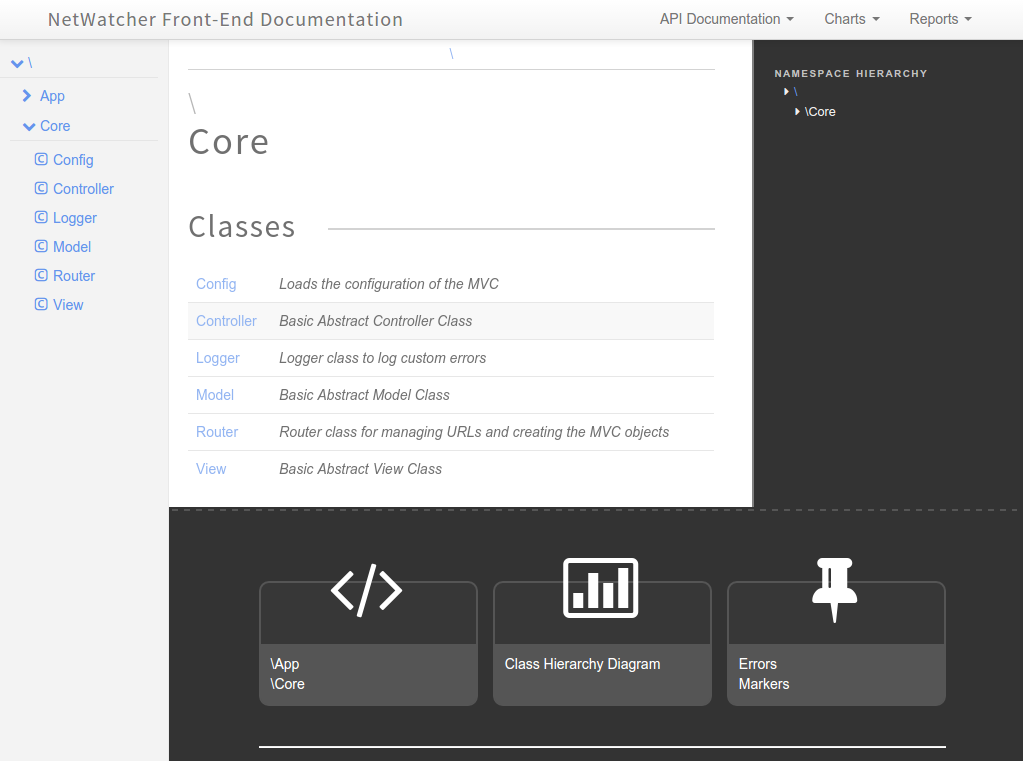
\includegraphics[width=0.95\textwidth,clip=true]{graphics/capturas/docs_frontend}
  \caption{Documentación web del \gls{front-end}.}
  \label{fig:captura:docsfrontend}
\end{figure} 
